\documentclass{beamer}
%
% Choose how your presentation looks.
%
% For more themes, color themes and font themes, see:
% http://deic.uab.es/~iblanes/beamer_gallery/index_by_theme.html
%
\mode<presentation>
{
  \usetheme{default}      % or try Darmstadt, Madrid, Warsaw, ...
  \usecolortheme{default} % or try albatross, beaver, crane, ...
  \usefonttheme{default}  % or try serif, structurebold, ...
  \setbeamertemplate{navigation symbols}{}
  \setbeamertemplate{caption}[numbered]
}

\usepackage[english]{babel}
\usepackage[utf8x]{inputenc}
\usepackage{graphicx}
\usepackage{wrapfig}
\usepackage{hyperref}

\title[Adversarial Autoencoders]{Adversarial Autoencoders}
\author{Jussi Martin}
%\institute{Where You're From}
\date{March 6, 2017}

\begin{document}

\begin{frame}
  \titlepage
\end{frame}

% Uncomment these lines for an automatically generated outline.
%\begin{frame}{Outline}
%  \tableofcontents
%\end{frame}

% \section{Introduction}
%
% \begin{frame}{Introduction}
%
% \begin{itemize}
%   \item Your introduction goes here!
%   \item Use \texttt{itemize} to organize your main points.
% \end{itemize}
%
% \vskip 1cm
%
% \begin{block}{Examples}
% Some examples of commonly used commands and features are included, to help you get started.
% \end{block}
%
% \end{frame}

\section{Introduction}

\begin{frame}{Introduction}
  We go through some of the main concepts presented in the paper \emph{Adversarial Autoencoders}
  written by Alireza Makhzani, Jonathon Shlens, Navdeep Jaitly, Ian Goodfellow, and Brendan Frey.


\end{frame}

\section{Adversarial Autoencoders (Definitions)}

\begin{frame}{Adversarial Autoencoders (Definitions)}
  Let $\mathbf{x}$ be the input vector and $\mathbf{z}$ latent code vector (hidden units) of an autoencoder
  with deep decoder an encoder. Let $p(\mathbf{z})$ be the distribution we want to impose
  on the latent vectors, $q(\mathbf{z}|\mathbf{x})$ be an encoding distribution, and
  $p(\mathbf{x}|\mathbf{z})$ the decoding distribution. Let also $p_{data}(\mathbf{x})$
  be the data distribution, $p(\mathbf{x})$ the model distribution.

  The encoding function of the autoencoder $q(\mathbf{z}|\mathbf{x})$ defines an
  \emph{aggregated distribution}
  \begin{equation*}
    q(\mathbf{z}) = \int q(\mathbf{z}|\mathbf{x})p_{data}(\mathbf{x})d\mathbf{x}
  \end{equation*}
on the latent vectors.

\end{frame}

\section{Adversarial Autoencoders (Principle)}

\begin{frame}{Adversarial Autoencoders (Principle)}
The adversarial autoencoder is an autoencoder that is regularized by matching the
aggregated posterior $q(\mathbf{z})$ to the given prior $p(\mathbf{z})$. This is done by attaching
an adversarial network on top of the latent vector $\mathbf{z}$, and allowing it to
guide $q(\mathbf{z})$ to converge towards $p(\mathbf{z})$. Meanwhile the autoencoder attemps
to minimize the reconstruction error.

The encoder of the autoencoder is also the generator of the adversarial network and
it tries to fool its discriminator in to thinking that the hidden code $q(\mathbf{z})$
comes
from the true distribution $p(\mathbf{z})$.

\end{frame}

\section{Architecture}

\begin{frame}{Architecture}

    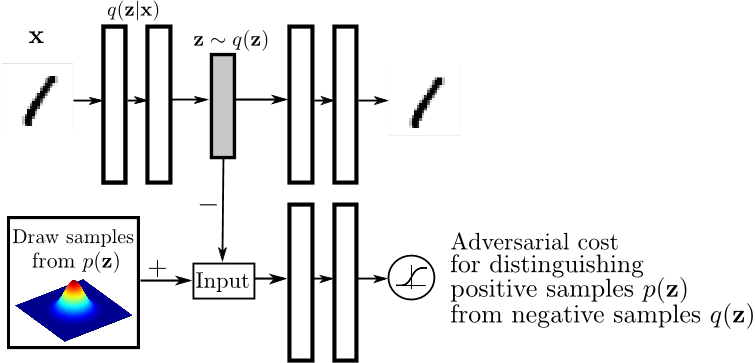
\includegraphics[width=1\textwidth]{1-Figure1-1.png}

\end{frame}

\section{Training}

\begin{frame}{Training}
  Both the adversarial network and the autoencoder are trained jointly with SGD in
  two phases -- the \emph{reconstruction} phase and the \emph{regularization} phase
  -- executed on each mini-batch.

  In the reconstruction phase, the autoencoder updates the encoder and the decoder
  to minimize the reconstruction error of the inputs.

  In the regularization phase, the adversarial network first updates its discriminative network
  to tell apart true samples ($z \sim p(\mathbf{z})$) from generated samples ($z \sim q(\mathbf{z})$).
  Then the adversarial network updates its generator (the encoder of the autoencoder) to fool
  the discriminator.

  When the training is finished, the decoder of the autoencoder will define a generative
  model that maps the imposed prior of $p(\mathbf{z})$ to the data distribution.
\end{frame}


\section{Different types of AAEs}

\begin{frame}{Different types of AAEs}

Accordig to the paper the adversarial autoencoder can be:
  \begin{itemize}
    \item Deterministic
    \item Gaussian Posterior
    \item Universal Approximator Posterior
  \end{itemize}
Howerver, the last approach might have some problems (see the comment in Dustin Tran's
blogpost), so we present only the first two here.
\end{frame}

\section{Deterministic}

\begin{frame}{Deterministic}
  Here we assume that $q(\mathbf{z}|\mathbf{x})$ is a deterministic function of
  $\mathbf{x}$. In this case the encoder is similar to the encoder of a standard
  autoencoder and the only source of stochasticity in $q(\mathbf{z})$ is the data
  distribution $p_{data}(\mathbf{x})$.

\end{frame}

\section{Gaussian Posterior}

\begin{frame}{Gaussian Posterior}
  Here we assume that $q(\mathbf{z}|\mathbf{x})$ is a Gaussian distribution whose
  mean and variance is predicted by the encoder network:
  \begin{equation*}
    \mathbf{z} =  \begin{pmatrix} z_1 \\ \vdots \\ z_n \end{pmatrix}
    \sim \begin{pmatrix}  \mathcal{N}(\mu_1(\mathbf{x}), \sigma_1(\mathbf{x})) \\
    \vdots \\  \mathcal{N}(\mu_n(\mathbf{x}), \sigma_n(\mathbf{x})) \end{pmatrix}.
  \end{equation*}
  In this case, the stochasticity in $q(\mathbf{z})$ comes from both the data-distribution and
  the Gaussian distribution at the output of the encoder. We can use the same re-parametrization
  trick of [Kingma and Welling, 2014] for back-propagation through the encoder network.


\end{frame}

% \section{Universal Approximator Posterior}
%
% \begin{frame}{Universal Approximator Posterior}
%   Adversarial autoencoders can be used to train $q(\mathbf{z}|\mathbf{x})$ as the
%   universal approximator of the posterior. Suppose the encoder network of the adversarial
%   autoencoder is the function $f(\mathbf{x}, \eta)$ that tkaes the input $\mathbf{x}$
%   and a random noise $\eta$ with a fixed distribution (e.g., Gaussian). We can sample ...
%
%   ...
%   \begin{eqnarray*}
%     q(\mathbf{z}|\mathbf{x}) &=& \int q(\mathbf{z}|\mathbf{x}, \eta)p_{\eta}(\eta)d\eta \\
%     \Rightarrow \quad q(\mathbf{z}) &=& \int \int q(\mathbf{z}|\mathbf{x}, \eta))p_{data}(\mathbf{x})p_{\eta}(\eta)d\eta d\mathbf{x}
%   \end{eqnarray*}
% ... (WAS THIS TOO OPTIMISTIC? see Dustin Tran's comments..)
%
% \end{frame}

\section{Comparison with Variational Autoencoders}

\begin{frame}{Comparison with Variational Autoencoders}
  Variational autoencoders try to minimize the upper bound
  \begin{equation*}
    E_{p_{data}(\mathbf{x})}[E_{q(\mathbf{z}|\mathbf{x})}[ -\log p(\mathbf{x}|\mathbf{z})]]
    - E_{p_{data}(\mathbf{x})}[KL( q(\mathbf{z}|\mathbf{x})\| p(\mathbf{z}))]
  \end{equation*}
  of $E_{p_{data(\mathbf{x})}}[- \log p(\mathbf{x})]$. Where the first term is the reconstruction error of the decoder
  $p(\mathbf{x}|\mathbf{z})$ trying to evaluate codes from the encoder $q(\mathbf{z}|\mathbf{x})$.
  The second term is the regularizer.

  The adversarial autoencoder's on the other hand uses
  \begin{equation*}
    JSD(p(\mathbf{z})\| q(\mathbf{z})) = \frac{1}{2}KL\Big( p(\mathbf{z})\Big\| \frac{p(\mathbf{z}) + q(\mathbf{z})}{2}\Big)
    +  \frac{1}{2}KL\Big( q(\mathbf{z})\Big\| \frac{p(\mathbf{z}) + q(\mathbf{z})}{2}\Big).
  \end{equation*}
  as a regularizer implicitly due to encoders adversarial training.
\end{frame}

\section{Further Topics}

\begin{frame}{Further Topics}

  \begin{itemize}
    \item Incorporating Label Information
    \item Semi-supervised AAEs
    \item Unsupervised Clustering
  \end{itemize}
  I might cover these in a later session.

\end{frame}


\section{Sources}

\begin{frame}{Sources}
  \begin{itemize}
    \item The paper: https://arxiv.org/pdf/1511.05644.pdf
    \item Dustin Tran's blogpost: http://dustintran.com/blog/adversarial-autoencoders
    \item Auto-Encoding Variational Bayes: https://arxiv.org/pdf/1312.6114.pdf
    \item Generative Adversarial Nets: https://arxiv.org/pdf/1406.2661.pdf
    \item Pictures from the paper: https://www.semanticscholar.org
  \end{itemize}
\end{frame}


% \section{Remarks}
%
% \begin{frame}{Remarks}
%   Since the adversarial autoencoders use adversarial networks in the training, there
%   are probably similar convergence issues involved as with regular adversarial networks.
%
%   Although not stated anywhere in the paper, the integrals with respect to the measure $p_{data}(\mathbf{x})d\mathbf{x}$
%   are to be understood as Monte Carlo integrals. Where the samples are the points in
%   the training set, drawn from the distribution $p_{data}(\mathbf{x})$. The distribution
%   $p_{data}(\mathbf{x})$ can be unknown, for example a distribution of all possible images of given size and content.
%
%
%
% \end{frame}


% \section{With Labels}
%
% \begin{frame}{With Labels}
%
%   \includegraphics[width=0.5\textwidth]{4-Figure3-1.png}
%
%   Alternatively it is also possible to add labels to the input.
%
% \end{frame}

% \section{Supervised Case}
%
% \begin{frame}{Supervised Case}
%
%   % \begin{wrapfigure}{r}{0.25\textwidth}
%   %          \vspace{-0.8cm}
%   %         \begin{center}
%   %        % \hspace{1cm}
%   %         \includegraphics[width=0.24\textwidth]{oma1.jpg} % REPLACE THIS
%   %         \vspace{-2cm}
%   %         \end{center}
%   %         %\vspace{-2cm}
%   %     \end{wrapfigure}
%   ...
% \end{frame}

% \section{Semi-supervised Case}
%
% \begin{frame}{Semi-supervised Case}
%
%   \includegraphics[width=0.4\textwidth]{8-Figure8-1.png}
%
%   ... (WRONG PICTURE? remove/change)
% \end{frame}

\end{document}
